\handoutpart{Ideas, and what to do}{This part turns the critique into a plan. It states the one idea that the draft contains, develops the two ideas that came out of the review (who keeps the gain from a tool, and the difference between more researchers and faster researchers), compares four ways of writing the paper, and sets out the recommended one with its tests, its fallback and a first month of work.}

\section{The ideas}\label{sec:ideas}

\subsection{One mechanism, four consequences}\label{sec:ideas-one}

The draft has one idea.

\begin{keybox}[The idea]
Entry is the margin on which science adjusts, and the price of entering a topic is reading its literature.
\end{keybox}

\begin{figure}[h]
\centering
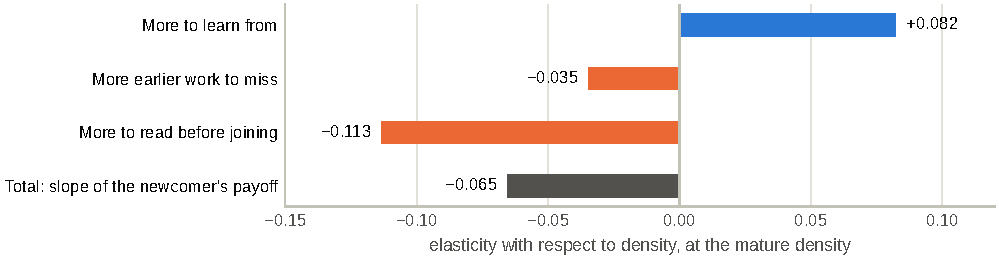
\includegraphics[width=\textwidth]{slope.pdf}
\caption{What makes a topic crowded for a newcomer. The slope of her payoff with respect to density at the calibrated mature density, split into its three parts. Computed from \texttt{code/results/calibration.json}.}
\label{fig:slope}
\end{figure}

Figure~\ref{fig:slope} is the model's own account of it. For someone inside a mature topic, one more paper is good news: the gain from having more to learn from ($+0.082$) exceeds the loss from having more earlier work to miss ($-0.035$). What makes the topic unattractive to someone outside is the reading she must do to get in ($-0.113$). The abstract says that reading has two jobs, to teach and to protect. It has a third, \emph{to admit}, and that is the one that carries the model. The protective job, on which most of the paper's empirical effort is spent, is the smallest of the three.

Four consequences follow from the idea. The draft presents them as separate results.

\begin{center}\small
\begin{tabularx}{\textwidth}{@{}P{1.75in}LP{1.25in}@{}}
\toprule
Consequence & Why it follows & Standing \\
\midrule
\textbf{1. More researchers widen science.} & A free researcher is indifferent between joining a topic and opening one. Extra researchers therefore open topics, and density barely moves. & Evidence in hand (Fact~1), to be repaired. \\
\textbf{2. Insiders earn a rent equal to the entry cost.} & Incumbents have paid; newcomers have not. Returns rise with density even where the topic is too crowded for a newcomer. & Theory solid; the gradient in Fact~2 is consistent with it. \\
\textbf{3. A tool's gain stays with whoever is not on the entry margin.} & The marginal entrant is always indifferent. What she gains is competed away into denser topics and longer reading. & A theorem that needs one repair and one measurement. \\
\textbf{4. Faster researchers are absorbed differently from more researchers.} & New researchers are free and go to the frontier at once. Existing researchers are insiders and stay; when they write more, their topics thicken. & Untested; the data are on disk. \\
\bottomrule
\end{tabularx}
\end{center}

The speed limit is the extreme case of the fourth consequence: a topic whose flow outruns what an outsider can read. Stated as a limit it never binds. Stated as a contrast between two kinds of growth it can be tested this year.

\subsection{Who keeps the gain from a tool}\label{sec:ideas-incidence}

\subsubsection{Three ways of not being on the margin}
The repair of \S\ref{sec:crit-lemma4} changes the incidence result from ``output equals the frontier'' to a statement about who is inframarginal. There are three ways of not being the marginal entrant:

\begin{center}\small
\begin{tabularx}{\textwidth}{@{}P{1.6in}P{1.4in}L@{}}
\toprule
Who & Statistic & Standing \\
\midrule
People who open topics and stay in them & the founders' share $\thF$ & Unmeasured. A first cut suggests it is above zero and below one half. \\
Cohorts that joined before entry was costly & their share of producer-years, $\iota$ (29\% in the stationary count) & Follows from how topics are born; rests on assumed rates of exit and obsolescence. \\
A frontier that is scarce & $\EE D$, from the volume elasticity & Measured, imprecisely. \\
\bottomrule
\end{tabularx}
\end{center}

\begin{ideabox}[A compact form of the repaired result]
For a tool that raises the payoff of everyone inside a topic (reading, learning), the share of the gain that survives entry is
\[
\Pi_L \;=\; 1-\frac{(1-\thF)\,(1-\EE D)\,\bigl[1-\iota\,(1+k)\bigr]}{1+\thF\,k},\qquad k=\frac{\eps_v}{|\eps_w|},
\]
and therefore
\[
\Pi_L\;\ge\;1-(1-\thF)\,(1-\EE D)\,(1-\iota).
\]
\emph{The gain is lost only on researchers who are marginal in all three senses.} The paper's theorem is the special case $\iota=0$, where the floor is $\EE D$.

The formula reproduces the four values established by the review: 0.167 and 0.736 for $\iota=0$ (the paper's numbers before rounding and shock size), and 0.495 and 0.87 with early cohorts. It is a local formula. It has not yet been checked against exact re-solved equilibria over the whole range, and at large $k$ it exceeds one, so it should organise the discussion and not carry a headline number.
\end{ideabox}

\begin{center}\small
\begin{tabularx}{0.9\textwidth}{@{}Lrrrr@{}}
\toprule
 & \multicolumn{4}{c}{Founders' time share $\omega$} \\
\cmidrule(l){2-5}
Volume elasticity $\EE$ & 0 & 0.25 & 0.5 & 0.75 \\
\midrule
\multicolumn{5}{@{}l}{\emph{As the paper states the theorem ($\iota=0$)}} \\
0.035 (the close-radius estimate) & 4\% & 42\% & 70\% & 90\% \\
0.15 (the paper's baseline) & 17\% & 50\% & 74\% & 91\% \\
0.27 (upper end) & 30\% & 58\% & 78\% & 93\% \\
\midrule
\multicolumn{5}{@{}l}{\emph{With early cohorts ($\iota=0.29$, $k=0.73$)}} \\
0.035 & 51\% & 71\% & 85\% & 95\% \\
0.15 & 58\% & 75\% & 87\% & 96\% \\
0.27 & 65\% & 79\% & 89\% & 96\% \\
\bottomrule
\end{tabularx}
\par\smallskip
\parbox{0.9\textwidth}{\footnotesize Share of a small reading gain that survives entry, from the local formula. The upper panel matches the grid recomputed in the review. The lower panel applies the factor $1-\iota(1+k)=0.505$ to the lost share; exact re-solves for 30\% shocks give 53\% and 85--88\% where it gives 58\% and 87\%.}
\end{center}

Two things stand out. With early cohorts, about half of a reading gain survives whatever the frontier and the founders do. And the answer depends much less on the unmeasured founders' share than the paper's range suggests: the band is 51--96\%, not 4--93\%.

\subsubsection{Capitalisation}
The distinctive economic point is what happens to a gain that reaches entrants and not the frontier. Density rises until the reading needed to join has grown enough to offset the gain. The marginal entrant ends up where she started. Insiders gain: for a reading tool, by $(\eps_\Gamma/|\eps_w|)\,h\approx1.7h$, more than one for one. In spatial economics a local improvement is capitalised into the price of land. Science has no land. The gain is capitalised into \emph{the queue to get in}, and it is collected by those who are already inside.

This gives predictions that a shock on the joiners' side could test: after such a shock, density and entry rise, incumbents' returns rise, and the lifetime returns of newcomers do not. No shock with outcomes exists yet; the review rule in computer science is the candidate, and it needs 2027 data.

\subsubsection{An accounting, not a ranking}
\begin{center}\small
\begin{tabularx}{\textwidth}{@{}P{1.5in}LL@{}}
\toprule
Tool & Where its gain goes & What decides the size \\
\midrule
Faster production & To everyone, explorers included, \emph{if} exploring speeds up with production. Lost to the extent that new topics are less fertile. & What explorers do; fertility depletion (unidentified). \\
Faster reading while producing & To insiders at once. After entry: to founders, to early cohorts, and through a scarcer frontier. & $\thF$, $\iota$, $\EE$. \\
Faster catch-up & To entrants at once. After entry: capitalised into denser topics; insiders gain; the frontier gains little. & The slopes $\eps_v$ and $\eps_w$. \\
\bottomrule
\end{tabularx}
\end{center}

What the paper needs here is measurement, not more theory: the founders' share; the share of a topic's output written by people who joined early; what the papers that open topics look like (how much they cite, how much their authors publish) compared with the papers that follow; and a range for the share of time spent reading (7\% to 16\%) carried through every table. With those in hand the nine-parameter calibration can be replaced in the main text by a table of sufficient statistics.

\subsection{More researchers or faster researchers}\label{sec:ideas-scale}

\subsubsection{The observation}
Science can grow in two ways: through more researchers, or through researchers who produce more. Until 2025 arXiv grew in the first way. In 2026 it began to grow in the second (\S\ref{sec:surge}). The paper's long-run result (Proposition~3) says the two are the same thing: density depends on the number of researchers $N$ and on their speed $a$ only through the product $Na$. Its own appendix says that on the way there they are very different, and the difference is a direct consequence of the idea in \S\ref{sec:ideas-one}.

\begin{center}\small
\begin{tabularx}{\textwidth}{@{}P{1.5in}LL@{}}
\toprule
 & More researchers & Faster researchers \\
\midrule
Who are they? & Newcomers, who are free. & Insiders, who have paid the entry cost. \\
Where does the extra output land? & At the frontier, at once: the marginal newcomer is indifferent (Remark~4). & In the topics the insiders are already in: every topic's flow rises at once (Appendix~B.8, Theorem~2(iv)). \\
What happens to density? & Barely moves ($\EE\approx0.15$). & Rises with output per researcher until entry and turnover undo it. \\
Why do insiders not move? & --- & Their payoff rises with density ($v'>0$) and they hold a premium (Proposition~5, Corollary~1). \\
In the long run & \multicolumn{2}{l}{The same: density depends on $Na$ only.} \\
\bottomrule
\end{tabularx}
\end{center}

\subsubsection{What the model predicts for 2026, corrected}

\begin{figure}[h]
\centering
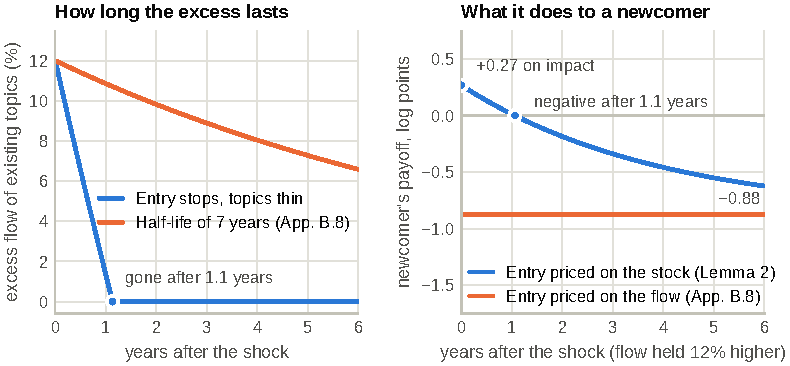
\includegraphics[width=\textwidth]{shock.pdf}
\caption{A production shock of 12\%, the size of the rise in papers per author in 2026, in the calibrated model. Left: the excess flow of existing topics if entry stops and topics thin through turnover, against the half-life stated in Appendix~B.8. Right: the change in a newcomer's payoff when entry is priced on the stock she must read (Lemma~2), against pricing on the flow (Appendix~B.8). Computed from \texttt{code/results/calibration.json}.}
\label{fig:shock}
\end{figure}

The appendix that contains this idea is wrong in two details, and both matter for what the 2026 data can show.

\textbf{How long the excess lasts.} The appendix says the spike decays ``with half-life $\ln2/\rho$'', about seven years. But in the model entry simply stops while topics are too dense, and they thin at the rate $\rho$ at which members leave. A 12\% excess is gone when $1.12\,e^{-\rho t}=1$, after $\ln(1.12)/\rho=1.1$ years. The window in which speed and scale differ is about a year at the assumed rate of exit, and shorter if real turnover is higher.

\textbf{What happens to entry.} The appendix says the newcomer's payoff falls at once. That prices entry on the flow. Lemma~2 prices it on the \emph{stock}, and the stock lags the flow: the day after the shock there is no more to read than the day before, and slightly more to learn from. Her payoff \emph{rises} by 0.27 log points on impact, turns negative after about a year, and ends 0.88 log points lower once the literature has built up.

So the model as written does not predict that entry stops in 2026. Three things follow.

\begin{enumerate}
\item \textbf{Testable now.} Where the extra papers of authors who sped up landed, and whether the flow of existing topics loads more on their incumbents' output than on growth in the number of authors. For a shock that builds up over the year, the reviewers' arithmetic gives a loading of 0.2 to 0.7 if entry stops, 0.9 to 1.0 if it does not respond, against about 0.15 for authors.
\item \textbf{A dated prediction, not a test this year.} Entry into the thickened topics falls in 2027, as their literature builds up.
\item \textbf{Signs, not magnitudes.} Every payoff change behind these predictions is below one log point, and entry in the model is infinitely elastic at indifference. Register the signs and the adding-up of extra flow and lower entry.
\end{enumerate}

\begin{critbox}[Settle the prediction before looking]
Three different predictions for 2026 are on the table: the appendix's (density one for one, a seven-year half-life), the corrected law of motion with entry priced on the flow (the excess absorbed in a year, entry falling at once), and the same with entry priced on the stock (entry unchanged for about a year). Until the authors derive one from a single law of motion, with the stock and the catch-up delay as states, either outcome can be read as support and the test cannot fail.
\end{critbox}

\subsubsection{Three views of the same regression}
The test becomes legible when set against two alternatives.

\begin{center}\small
\begin{tabularx}{\textwidth}{@{}P{2.1in}LL@{}}
\toprule
 & \multicolumn{2}{c}{Response of local density to growth in \ldots} \\
\cmidrule(l){2-3}
View & the number of authors & papers per author \\
\midrule
A fixed idea space & at the benchmark (0.5--0.8) & at the benchmark \\
Free choice of topics, no entry cost (everyone mobile) & low ($\EE$) & low ($\EE$) \\
\textbf{This model} (entry costs reading; insiders stay) & \textbf{low} ($\EE$) & \textbf{high at first, falling to $\EE$} \\
\bottomrule
\end{tabularx}
\end{center}

The first row is rejected by Fact~1. The contrast between the second and third rows is the footprint of the entry cost, and it is what 2026 can show.

\subsubsection{Why this is the natural headline, and its limits}
It is the honest reading of the paper's best fact, which is about scale. It uses the first production shock in the data. It speaks to the question people ask about artificial intelligence: is growth through faster researchers different from growth through more researchers? It needs no founders' share and no calibration for its first half. And it degrades well: if speed turns out to look like scale, the paper keeps a second fact (a rise in output per author did not thicken topics either) and falls back on the entry margin and incidence.

Its limits are real. ``People who write more write near their earlier work'' is what any topic-specific skill predicts; it does not show that the entry cost is \emph{reading}. The stakes inside the model are small. The shock is nine months old, still building, and measured with text similarity in the year in which the wording of abstracts changed. \S\ref{sec:tests} takes these one by one.

\subsection{Other ideas worth keeping}\label{sec:ideas-other}

\begin{enumerate}
\item \textbf{Differences in entry barriers would produce the falling arm.} If topics differ in how costly they are to enter, easy-to-enter topics are dense and their rents are competed away, and the cross-section traces the payoff curve itself (\S\ref{sec:crit-calib}).
\item \textbf{The barrier signature.} Holding a topic's recent flow fixed, a larger stock of older papers should go with fewer newcomers, higher returns for incumbents and no extra exit. A topic that is merely exhausted predicts fewer newcomers, \emph{lower} returns and more exit. Three outcomes, opposite signs. It is the only cheap evidence that the cost of entry is the literature.
\item \textbf{What do the people who open topics do?} Compare the reference lists and the output of papers that open a cluster with those of papers that follow. This turns the ranking of tools from an assumption into a measurement.
\item \textbf{Put fertility depletion inside the theorem} and report results as a function of it, instead of in an appendix that reverses the main corollary.
\item \textbf{Derive the admission standard.} Let a newcomer need coverage $\bar c$ of the stock, which gives a limit of $b_c/\bar c$, and show what survives if the reading required is concave in the stock.
\item \textbf{Add the catch-up delay to the law of motion}, with people who are still reading as a state variable.
\item \textbf{Measure the rates instead of assuming them.} Turnover of authors in topic cells gives $\rho$; the age profile of the references newcomers cite gives $\delta$; cell survival gives $\xi$. The decay rate $\delta$ is the one parameter that could move topics close to the speed limit.
\item \textbf{Entry through apprenticeship.} The model has solo researchers. Much real entry comes with an incumbent co-author, which lowers the reading cost. The share of entry of this kind is measurable.
\item \textbf{Say ``a sunk entry cost'' unless reading is shown.} The results hold for any cost that rises with the stock and that insiders have already paid. The word ``reading'' has to be earned by the stock gradient in item~2.
\item \textbf{State the small magnitudes as findings.} Duplication is pinned by entry, the static misallocation is about 1\%, crowding explains little of stepping on toes. The feared effects are small, and the theory explains why.
\item \textbf{Readership deserves a model.} The literal meaning of the title is that papers are produced faster than they can be read. Proposition~8 only relabels output. A model in which a paper's value comes from being read would make this a result, and it is a different paper.
\item \textbf{Separate rents from sorting.} Able researchers may sort into dense topics. Interacting density with early-career citations distinguishes this from an entry rent.
\item \textbf{Theory of neighbourhoods, not of persons.} State the results for densities and drop ``first follower'' and ``one entrant at a time'', or rescale so that a topic has tens of members.
\item \textbf{A short format.} Two facts, a four-page model, one test. The reviewers judged that this material fits a short paper better than a 40-page model with a calibration.
\end{enumerate}
